In the present work, the Bitcoin market price prediction is treated as a binary classification problem. To the best knowledge of the author of the present paper, there is no standard binary classification dataset of the Bitcoin market price direction available. Hence, this Section is concerned with the development of such a binary classification dataset starting from time series data on the Bitcoin  market price and other measures, in Subsection~\ref{subsec:time_series_data}. The transformation into a binary classification dataset is treated in Subsection~\ref{subsec:bin_class_data}.

\subsection{Bitcoin Time Series Data}\label{subsec:time_series_data}

The Bitcoin time series data is taken from the Blockchain.com API, see  \cite{Data}. In the present work, the time period from \date{01 September 2011} to \date{15 June 2021} is considered. The starting date of the time period is chosen such that there were already some established cryptocurrency exchanges that allow a reliable determination of the Bitcoin market price.\\

The measures that are obtained from the Blockchain.com API are displayed in Fig.~\ref{fig:blockchain.api} as a function of the date. All measures are day-by-day time series for a total of $3576$ days corresponding to the considered time period mentioned above. The most important measure is the Bitcoin market price that reports the value of one Bitcoin in the fiat currency USD. In the present work, USD is chosen as the reference currency as is usually done for financial assets. The market cap describes the value of all Bitcoins that have ever been mined at the current market price. It is the product of the total number of Bitcoins and the current market price. Another measure is the number of transactions per day, i.e. how often Bitcoins are transferred on each day. The transaction volume reported in Bitcoins (BTC) is the total worth of these transactions. The average blocksize in megabyte (MB) is a measure for the number of transactions contained in each block. In combination with the relative difficulty of the mathematical task to mine new blocks, this reports how much computing power has to be applied to mine a new block. The hash rate expressed in $\mathrm{EH} / \mathrm{s}$ (\enquote{Exahashes per second}) is an estimate of the total computing power that all mining entities are applying on each day. Finally, the miner's revenue is the sum of the reward that miners obtain for mining a new block and the transaction fees per block. It reports how miners are rewarded for their computational efforts.\\

From Fig.~\ref{fig:blockchain.api}, it seems that the market price and the market cap reveal the exact same development. The reason for this is that the market price is the USD value of one Bitcoin, and the market cap the USD value of all available Bitcoins. In other words, the market cap is the market price multiplied by the total number of available Bitcoins. Thus, the market cap is not useful to predict the Bitcoin market price of tomorrow if the market price of today and the past days is already considered. Also, the block difficulty and the miner's revenue show a time series similar to the market price. In contrast, the transaction volume appears to be fluctuating with a constant magnitude without any trend over the time. From this perspective, also the transaction volume cannot be used to predict the market price because it contains only time independent information.\\

These qualitative impressions can be quantified by plotting the correlation matrix of the different time series, as in Fig.~\ref{fig:correlation_matrix}. Indeed, the market cap has a correlation of $1$ with the market price. In addition, the miner's revenue and the difficulty have a correlation coefficient of $0.8$ or higher with the market price. Thus, these measures are not further considered since they are not expected to be useful for the prediction of tomorrow's Bitcoin market price because they simply follow the development of the Bitcoin market price. Furthermore, the transaction volume - as already observed above - is only weakly correlated to the market price and the other measures. Hence, also the transaction volume is not helpful for the prediction of the Bitcoin market price and is dropped.\\

An overview of the remaining measures can be found in Fig.~\ref{fig:all_vs_all}. The Figure reports a scatterplot matrix of the four remaining measures that appear to be useful for the prediction of tomorrow's Bitcoin market price direction. The diagonal contains the densities of the measures. In addition, Pearson's correlation coefficients - the same as in Fig.~\ref{fig:correlation_matrix} - are stated. As the correlation coefficients are computed from time series data, the measures are not only moderatly correlated with the Bitcoin market price but they are also correlated among themselves. 

\begin{figure}[h!]
  \centering
  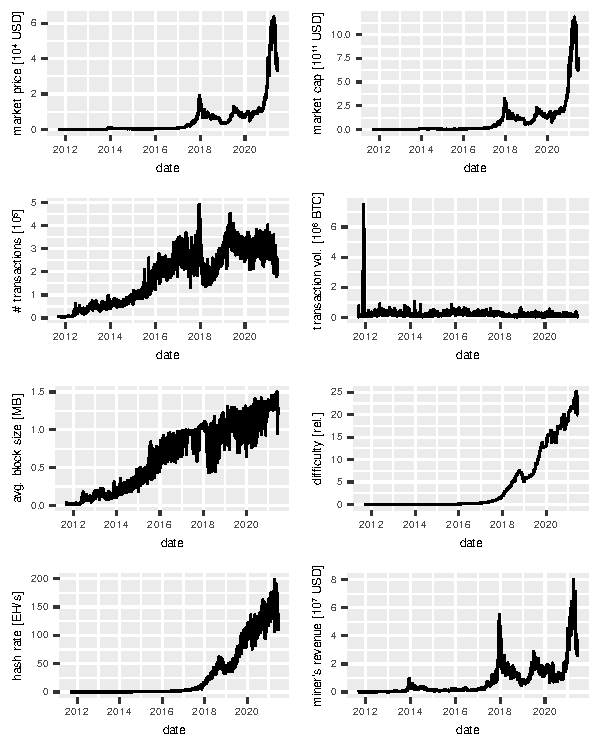
\includegraphics[width=1\textwidth]{data.pdf}
  \caption{Bitcoin day-by-day time series data obtained from the Blockchain.com API, see \cite{Data}. The time series of the Bitcoin market price and the other displayed measures are reported for the time period from \date{01 September 2011} to \date{15 June 2021}. This is a total of $3576$ days. The different measures are explained in the main text.}
  \label{fig:blockchain.api}
\end{figure}

\begin{figure}[h!]
  \centering
  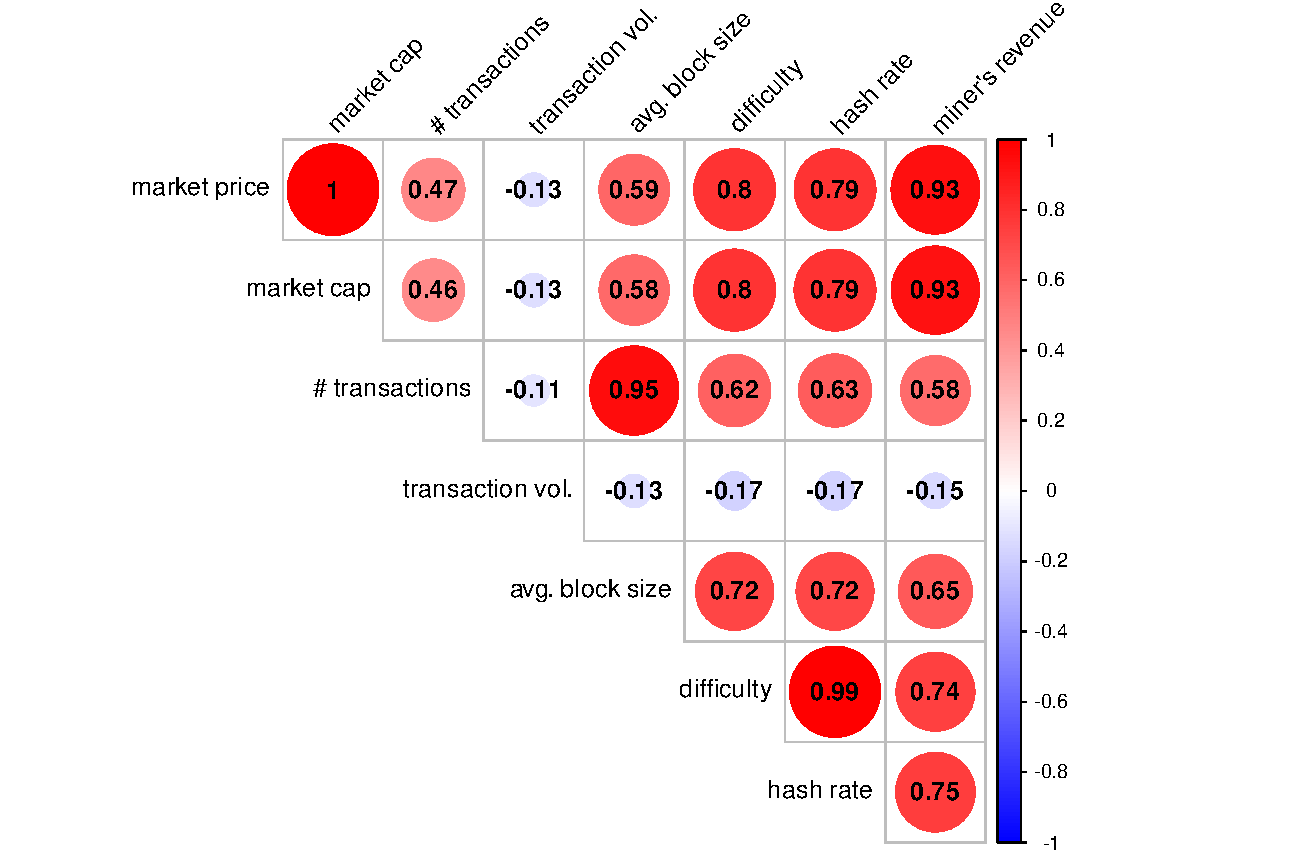
\includegraphics[width=0.72\textwidth]{cor_mat.pdf}
  \caption{Pearson's correlation matrix of the time series from Fig.~\ref{fig:blockchain.api}. As the market cap, the difficulty, and the miner's revenue have a correlation coefficient of $0.8$ or higher, these measures are not expected to be useful for the prediction of tomorrow's Bitcoin market price. In contrast, the transaction volume is weakly correlated with the Bitcoin market price and the other measures, and does not contain any time-dependent information. Thus, it is also dropped. An overview of the remaining measures can be found in Fig.~\ref{fig:all_vs_all}.}
  \label{fig:correlation_matrix}
\end{figure}

\begin{figure}[h!]
	\centering
	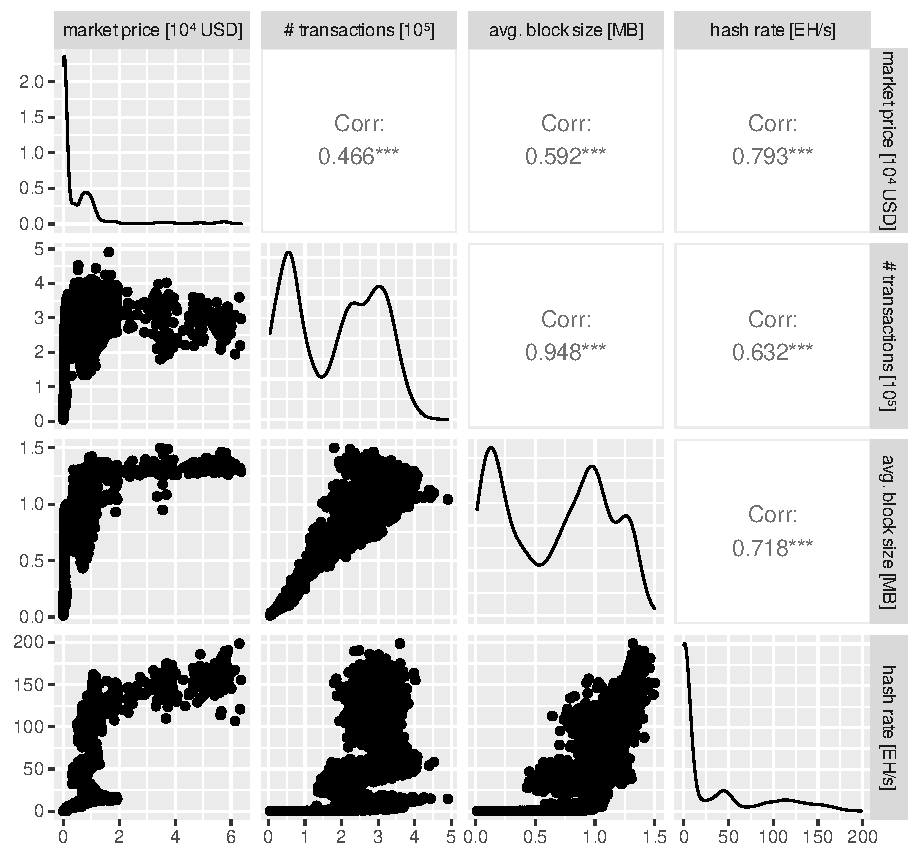
\includegraphics[width=0.72\textwidth]{all_vs_all.pdf}
    \caption{Scatterplot matrix of the remaining four measures selected from the original time series dataset in Fig.~\ref{fig:blockchain.api} that appear to be useful for the prediction of tomorrow's Bitcoin market price. The line plots on the diagonal are the densities of the respective measures. The upper righthand part of the Figure reports Pearson's correlation coefficients - the same as in Fig.~\ref{fig:correlation_matrix} - between the measures.}
    \label{fig:all_vs_all}
\end{figure}

\subsection{Transformation to Binary Classification Dataset}\label{subsec:bin_class_data}

In order to obtain a binary classification dataset for the prediction of tomorrow's direction of the Bitcoin market price, the four selected time series including the market price from the previous Subsection are used.\\

First of all, Fig.~\ref{fig:autocorrelation} displays the autocorrelation of the Bitcoin market price as a function of the lag. The autocorrelation plot gives an idea on the number of days in the past including today that might contain information on tomorrow's Bitcoin price. As can be seen in the Figure, the autocorrelation drops below a value of $0.5$ after a lag of about $100$ days. It is expected that this period of time might be useful for the prediction of tomorrow's Bitcoin market price.

\begin{figure}[h!]
	\centering
	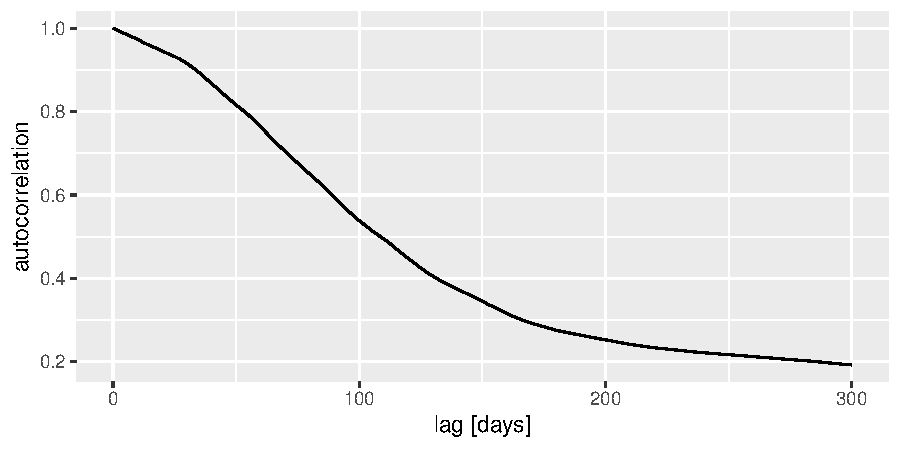
\includegraphics[width=0.8\textwidth]{autocorrelation.pdf}
    \caption{Autocorrelation of the Bitcoin market price. The autocorrelation drops below a value of $0.5$ after a lag of about $100$ days. This information is used in the construction of the binary classification dataset by applying the moving window method, see the example structure in Fig.~\ref{fig:example}.}
    \label{fig:autocorrelation}
\end{figure}

For the construction of the binary classification dataset, the \textit{moving window approach} (also called sliding window approach) is applied. The starting point of the moving window approach is to consider the first $m$ days of the four selected time series presented in the last Subsection. This leads to four new time series of length $m$ from date $t_{m-2}$ until $t_{+1}$, where $t_{+1}$ is the date of \enquote{tomorrow}, $t_0$ is the date of \enquote{today}, and so on. The dates from $t_{m-2}$ until $t_{0}$ are considered as the features of the supervised learning approach, while the date $t_{+1}$ is transformed into a label. In the present work, the label is \enquote{1} if the Bitcoin market price on date $t_{+1}$ is larger than on date $t_0$, and as \enquote{0} if it is lower. In the following, the notations \enquote{1} and \enquote{up}, and \enquote{0} and \enquote{down} are used interchangeably. This combination of features and label is the first example of the binary classification dataset. After that, the starting date of the window is shifted by one day, and another example is constructed. This process is repeated until the last date $t_{+1}$ of the moving window coincides with the last day of the overall time series. The result is a set of labeled examples as depicted in Fig.~\ref{fig:example} that together build the binary classification dataset. In the present work, based on the autocorrelation plot from Fig.~\ref{fig:autocorrelation}, a window length of $m=100$ is chosen. 

In applying the moving window approach, for each window, the four time series - before considering them as features - are standardized using the min-max-transformation
\begin{align*}
	\hat{x}_t = \frac{x_t - \min_{t' \in \{t_{m-2}, \dots ,t_{0}\}}(x_{t'})}{\max_{t' \in \{t_{m-2}, \dots ,t_{0}\}}(x_{t'}) - \min_{t' \in \{t_{m-2}, \dots ,t_{0}\}}(x_{t'})},
\end{align*}
where $\hat{x}_t \in [0,1]$ is the standardized window time series, and $x_t$ the intial window time series (e.g. the Bitcoin market price). Of course, the date is $t \in \{t_{m-2}, \dots ,t_{0}\}$ because the date $t_{+1}$ is used for the label, and is not included in the features. \\

In total, $3477$ examples are generated using the moving window technique. \\

Finally, the binary classification dataset constructed using the moving window approach is split into a training and a test part, after the $3477$ examples have been shuffled randomly. The training set contains \SI{80}{\percent} of the examples in the original dataset, while the remaining \SI{20}{\percent} are the test set. This leads to a training set with $2782$ examples, and a test set with $695$ examples. Both sets are slightly unbalanced towards an increasing Bitcoin market price, see Fig.~\ref{fig:test}.

\begin{figure}[h!]
	\centering
	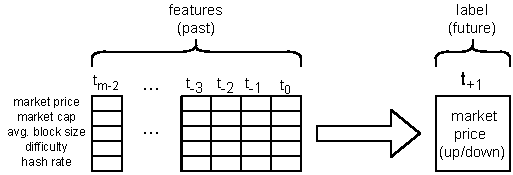
\includegraphics[width=\textwidth]{moving_window.pdf}
    \caption{Structure of the examples in the binary classification dataset obtained by applying the moving window approach on the four selected time series. There are $m-1$ dates for each selected time series that are treated as features. The label of each example is the direction of tomorrow's Bitcoin market price, and is used as the label. In the present work, based on the autocorrelation plot from Fig.~\ref{fig:autocorrelation}, $m=100$ is used as the length of the moving window.}
    \label{fig:example}
\end{figure}

\begin{figure}[h!]
\centering
\begin{subfigure}{.5\textwidth}
  \centering
  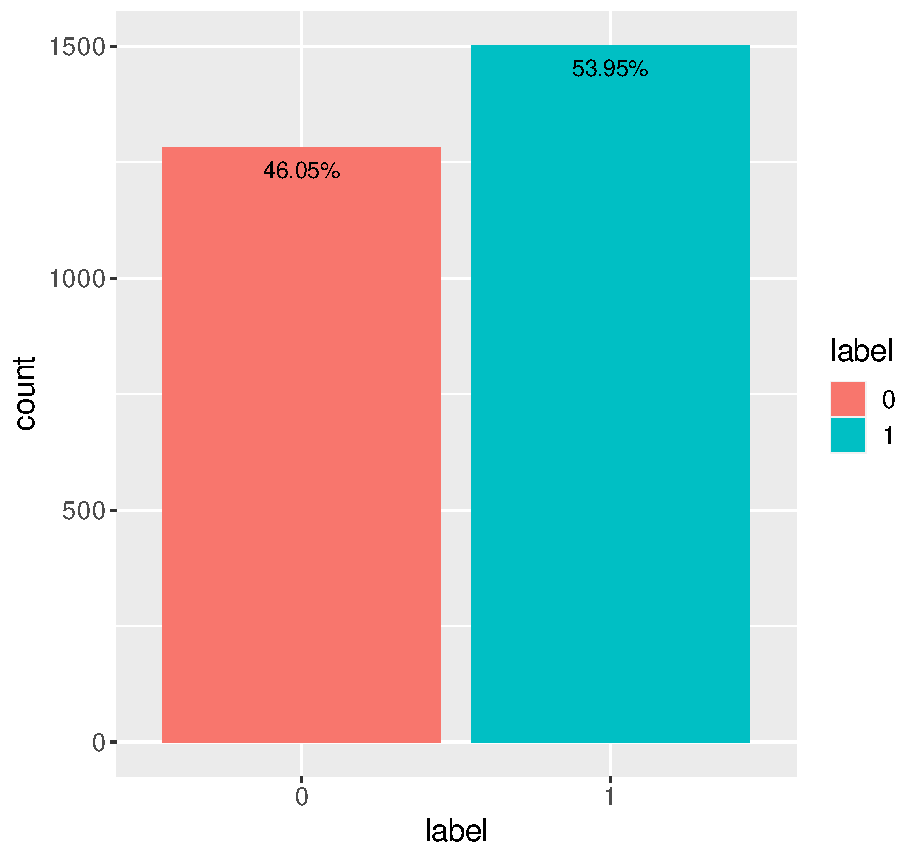
\includegraphics[width=\linewidth]{balance_train.pdf}
  \caption{training examples}
  \label{fig:sub1}
\end{subfigure}%
\begin{subfigure}{.5\textwidth}
  \centering
  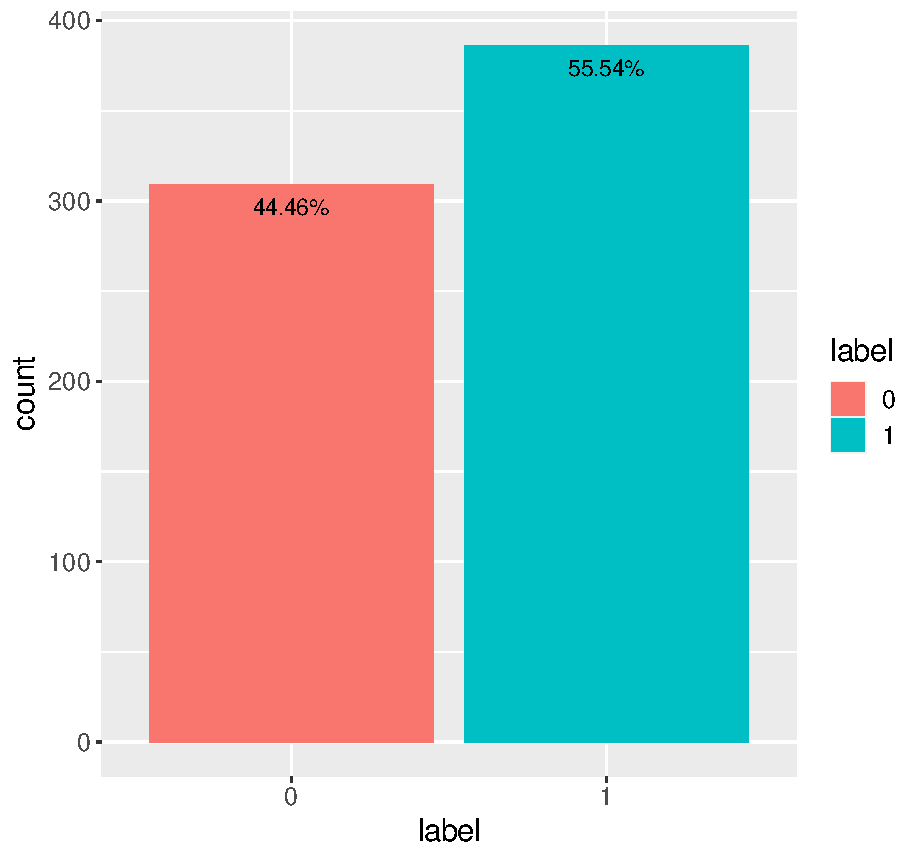
\includegraphics[width=\linewidth]{balance_test.pdf}
  \caption{test examples}
  \label{fig:sub2}
\end{subfigure}
\caption{Split of the binary classification dataset into a training (\SI{80}{\percent}) and a test (\SI{20}{\percent}) part. Both sets are slightly unbalanced towards an increasing Bitcoin market price.}
\label{fig:test}
\end{figure}